%%%%%%%%%%%%%%%%%%%%%%%%%%%%%%%%%%%%%%%%%%%%%%%%%%%%%%%%%%%%%%%%%%%%%%%%%%%%%%%%%%%%%%%%%%
% Ceci est le template à utiliser pour les milestones des projets d'INFO0947.            %
%                                                                                        %
% Vous devez décommenter et compléter les commandes introduites plus bas (intitule, ...) %
% avant de pouvoir compiler le fichier LaTeX.                                            %
%                                                                                        %
% Le PDF produit doit avoir la forme suivante: grpID_ProjetX_MilestoneY.pdf              %
% où:                                                                                    %
%   - grpID est votre identifiant de groupe (cfr. eCampus)                               %
%   - X est le numéro du projet (1 pour Construction, 2 pour TAD)                        %
%   - Y est le numéro du milestone (1 ou 2)                                              %
%%%%%%%%%%%%%%%%%%%%%%%%%%%%%%%%%%%%%%%%%%%%%%%%%%%%%%%%%%%%%%%%%%%%%%%%%%%%%%%%%%%%%%%%%%


% !TEX root = ./main.tex
% !TEX engine = latexmk -pdf
% !TEX buildOnSave = true


\documentclass[a4paper, 11pt, oneside]{article}

\usepackage[utf8]{inputenc}
\usepackage[T1]{fontenc}
\usepackage[T2A]{fontenc}
\usepackage[french]{babel}
\usepackage{array}
\usepackage{shortvrb}
\usepackage{listings}
\usepackage[fleqn]{amsmath}
\usepackage{amsfonts}
\usepackage{fullpage}
\usepackage{enumerate}
\usepackage{graphicx}             % import, scale, and rotate graphics
\usepackage{subfigure}            % group figures
\usepackage{alltt}
\usepackage{url}
\usepackage{indentfirst}
\usepackage{eurosym}
\usepackage{listings}
\usepackage{color}
\usepackage[table,xcdraw,dvipsnames]{xcolor}


%%%%%%%%%%%%%%%%% TITRE %%%%%%%%%%%%%%%%
\newcommand{\intitule}{Milestone 2}
\newcommand{\GrNbr}{33}
\newcommand{\PrenomUN}{Pavlov}
\newcommand{\NomUN}{Aleksandr}
\newcommand{\PrenomDEUX}{Gendebien}
\newcommand{\NomDEUX}{Alexandre}


%%%%%%%% ZONE PROTÉGÉE : MODIFIEZ UNE DES DIX PROCHAINES %%%%%%%%
%%%%%%%%            LIGNES POUR PERDRE 2 PTS.            %%%%%%%%
\title{INFO0947: \intitule}
\author{Groupe \GrNbr : \PrenomUN~\textsc{\NomUN}, \PrenomDEUX~\textsc{\NomDEUX}}
\date{}
\begin{document}

\maketitle
%%%%%%%%%%%%%%%%%%%% FIN DE LA ZONE PROTÉGÉE %%%%%%%%%%%%%%%%%%%%


%%%%%%%%%%%%%%%% MILESTONE %%%%%%%%%%%%%%%
\section{Invariants}
%%%%%%%%%%%%%%%%%%%%%

\subsection{Invariant 1}



\begin{figure}[h]
    \centering
    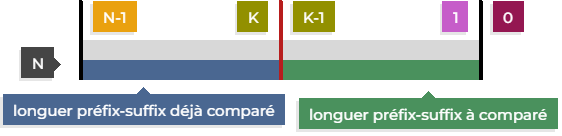
\includegraphics[width=0.5\textwidth]{inv1.png}
    \caption{Invariant Graphique 1}
\end{figure}

\textbf{Invariant Formel:}

\[ 0 < k < N \]

\subsection{Invariant 2}


\begin{figure}[h]
    \centering
    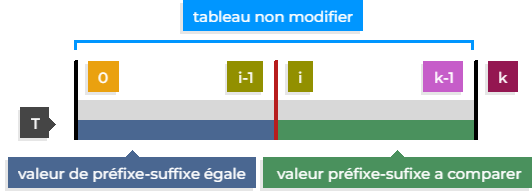
\includegraphics[width=0.5\textwidth]{invariant_T_2.png}
    \caption{Invariant Graphique 2}
\end{figure}

\textbf{Invariant Formel:}

\[ T = T_0 \land k = k_0 \]
\[ \land \]
\[ 0 \leq i < k \]





% \[ \land \]
% \[ T[i] = T[N - k + i] \]

% \[
% N \geq 0 \land \forall i \cdot (i \in 0 \dots N-1 \Rightarrow T[i] \in \mathbb{Z})
% \]
% \[
% \operatorname{prefixe\_suffixe}(T, N) \equiv \max\{k \mid k \in 0 \dots N-1 \land \forall i \cdot (i \in 0 \dots k - 1 \Rightarrow T[i] = T[N-k+i])\}
% \]



%%%%%%%%%%%%%%%%%%%%%%%

%%%%%%%%%%%%%%%%%%%%%%%%%%%%%%%%%%%%%%%%%%%%%%%%%%%%%%%%%%%%%%%%%%%%%%%%%%%%%%%%%%%%%%%%%%
% Dans cette section, vous pouvez rédiger les questions que vous avez sur le projet ou   %
% formuler ce qui reste incompris pour vous.                                             %
%                                                                                        %
% Nous en discuterons lors de la rencontre feedback sur votre production pour le         %
% milestone                                                                              %
%%%%%%%%%%%%%%%%%%%%%%%%%%%%%%%%%%%%%%%%%%%%%%%%%%%%%%%%%%%%%%%%%%%%%%%%%%%%%%%%%%%%%%%%%%

\end{document}
